%%%%%%%%%%%%%%%%%%%%%%%%%%%%%%%%%%%%%%%%%%%%%%%%%%%%%%%%%%%%%%%%%%%%%
% LaTeX Template: Relatório de LSD
% 
%%%%%%%%%%%%%%%%%%%%%%%%%%%%%%%%%%%%%%%%%%%%%%%%%%%%%%%%%%%%%%%%%%%%%%

\documentclass[12pt]{article}
\usepackage[portuguese]{babel}
\usepackage[a4paper]{geometry}
\usepackage{graphicx, wrapfig, subcaption, setspace, booktabs}
\usepackage[T1]{fontenc}
\usepackage[utf8]{inputenc}
\usepackage[font=small, labelfont=bf]{caption}
\usepackage{url, lipsum}
\usepackage{hyperref}
\usepackage{xcolor}
\usepackage[portuguese]{babel}
\usepackage{enumitem}
\usepackage{algorithm}
\usepackage{minted}
\usepackage{indentfirst}
\usepackage{float}
\usepackage[table]{xcolor}
\usepackage[usenames,dvipsnames]{xcolor}
\usepackage[bottom]{footmisc}
\usepackage[document]{ragged2e}
\usepackage{fancyvrb}
\usepackage{caption}
\usepackage{subcaption}
\usepackage{hhline}
\usepackage{circuitikz}
\onehalfspacing
\usepackage{geometry}[]
\geometry{margin=.8in,bottom=1in}

\graphicspath{{images/}}


\usepackage{fancyhdr}

\fancypagestyle{geral}{
  \fancyhf{}
  \renewcommand{\footrulewidth}{0.3pt}
  \fancyhead[R]{\rule[-5mm]{0pt}{2ex}\nouppercase{\leftmark}}
  \fancyfoot[C,RE]{\rule[3mm]{0pt}{2ex}\textbf{\thepage}}
}

\fancypagestyle{firstpage}{
  \fancyhf{}
  \renewcommand{\footrulewidth}{0.3pt}
  \fancyhead[R]{\rule[-5mm]{0pt}{2ex}1\hspace{4mm}Objetivo}
  \fancyfoot[C,RE]{\rule[3mm]{0pt}{2ex}\textbf{\thepage}}
}

\fancypagestyle{referencias}{
  \fancyhf{}
  \renewcommand{\footrulewidth}{0.3pt}
  \fancyhead[R]{\rule[-5mm]{0pt}{2ex}Referências}
  \fancyfoot[C,RE]{\rule[3mm]{0pt}{2ex}\textbf{\thepage}}
}

\fancypagestyle{remissivo}{
  \fancyhf{}
  \renewcommand{\footrulewidth}{0.3pt}
  \fancyhead[R]{\rule[-5mm]{0pt}{2ex}C\hspace{4mm}Índice Remissivo}
  \fancyfoot[C,RE]{\rule[3mm]{0pt}{2ex}\textbf{\thepage}}
}


\begin{document}


   
\begin{titlepage}
    \hspace{-1.5cm}
    
\includegraphics[scale=0.5]{logo_DEETC_cor_completo.png}\\
    \begin{center}
    \large
        Licenciatura em Engenharia Informática e de Computadores e\\
        Licenciatura em Engenharia Informática, Redes e Telecomunicações\\
        
    \vspace{0.5cm}
    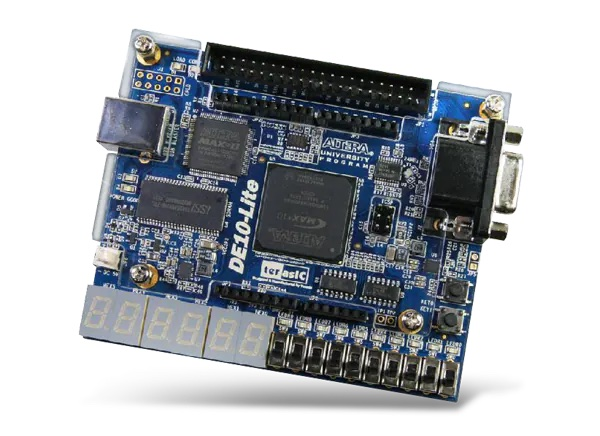
\includegraphics[width=10cm]{de10-lite.jpg}\\
    \vspace{0.5cm}

    \LARGE \uppercase{Relatório do} 1º \uppercase{Trabalho}\\
    \textbf{Circuitos Combinatórios}
    \end{center}

    \vspace{1cm}

Trabalho realizado por:

\begin{itemize}[label={}]
    \setlength\itemsep{0.5mm}
    \item \textbf{Gustavo Costa | Nº 52808}
    \item \textbf{Rafael Pereira | Nº 52880}
\end{itemize}

Turma: \textbf{LEIC15D}


Docente: \textbf{Prof.º Mário Véstias}

\begin{center}
Lógica e Sistemas Digitais (LSD)

2024 / 2025 Semestre de Inverno

\end{center}

\end{titlepage}

\renewcommand{\contentsname}{Conteúdo \vspace{5mm}\hrule}

\setcounter{page}{1}
\pagenumbering{roman} % Arabic/Indic page numbers
\addcontentsline{toc}{section}{\protect\numberline{}Índice}
\tableofcontents
\newpage

%-------------------------------------------------------------------------------
% BODY
%-------------------------------------------------------------------------------

\pagestyle{firstpage}
\pagenumbering{arabic} % Arabic/Indic page numbers
\setcounter{page}{2}

\section{Objetivo} \label{obj}
\hrule
\vspace{0.5cm}
\justifying


Este trabalho consiste em projetar, simular e implementar um circuito combinatório utilizando \textbf{VHDL} estrutural na placa \textbf{DE10-Lite da Intel}. O circuito irá verificar se o número de entradas ativas é \textbf{ímpar}, e, caso se verifique, irá \textbf{ativar a saída de paridade} (P). Se todas as entradas estão inativas, irá \textbf{ativar a saída zero }(Z). Para tal, será utilizada uma abordagem \textbf{hierárquica}, subdividindo o problema em blocos lógicos (3 blocos \textbf{PZ4} e 1 \textbf{AND} de 3 entradas) que verificam \textbf{paridade e zero} para subconjuntos das entradas, culminando na verificação de todas as 10 entradas da placa.


\section{Descrição do Circuito a Projetar}
\hrule

\vspace{0.5cm}
O circuito a ser projetado é responsável por analisar as 10 entradas (inputs), que verifica se:

\begin{enumerate}[label={-}]
    \item O número de entradas ativas é \textbf{ímpar}, o que torna a saída da paridade \textbf{ativa (valor 1)};
    \item O número de entradas ativas é \textbf{par}, o que torna a saída da paridade \textbf{inativa (valor 0)};
    \item Todas as entradas estão \textbf{inativas}, o que torna saída de zero \textbf{ativa (valor 1)};
    \item Pelo menos uma das entradas está \textbf{ativa}, o que torna a saída de zero \textbf{inativa (valor 0)}.
\end{enumerate}

\vspace{2mm} O circuito (PZ10) é constituído por \textbf{10 entradas} (I0, I1, I2, I3, I4, I5, I6, I7, I8 e I9), que correspondem a 10 botões da nossa placa de teste \textit{DE10-Lite} da Intel e por \textbf{2 saídas} (P e Z), que serão interpretadas através de 2 LEDs da mesma placa.

\vspace{2mm} Este circuito deve ser montado utilizando blocos funcionais que implementam um \textbf{verificador de paridade} e um \textbf{verificador de zero}, ambos com 4 entradas cada.



\begin{figure}[H]
\centering
\begin{circuitikz}
    \draw
    (0,0) node[anchor=east] {I0} -- (1,0)
    (0,-0.5) node[anchor=east] {I1} -- (1,-0.5)
    (0,-1) node[anchor=east] {I2} -- (1,-1)
    (0,-1.5) node[anchor=east] {I3} -- (1,-1.5)
    (0,-2) node[anchor=east] {I4} -- (1,-2)
    (0,-2.5) node[anchor=east] {I5} -- (1,-2.5)
    (0,-3) node[anchor=east] {I6} -- (1,-3)
    (0,-3.5) node[anchor=east] {I7} -- (1,-3.5)
    (0,-4) node[anchor=east] {I8} -- (1,-4)
    (0,-4.5) node[anchor=east] {I9} -- (1,-4.5)

    % Caixa do PZ10
    (1,0.5) rectangle (3,-5)

    % Saídas P e Z
    (3,-2) -- (4,-2) node[anchor=west] {P}
    (3,-2.5) -- (4,-2.5) node[anchor=west] {Z}

    % Nome da Caixa
    (2,-2.25) node {PZ10};
\end{circuitikz}
\caption{Diagrama disponibilizado no enunciado do circuito \textit{PZ10}}
\end{figure}

\newpage
\pagestyle{geral}

\section{Desenvolvimento do Projeto}
\hrule
\vspace{0.5cm}
% (como é que chegamos a esta conclusão)
Inicialmente, analisámos o circuito que nos foi pedido de acordo com o guião disponibilizado na plataforma \textit{Moodle}, pelo professor Mário Véstias, e percebemos de que maneira iria se formular. A escolha do operador lógico \textbf{XNOR} baseou-se pelo facto de este operador apresentar apenas um output ativo, se e só se, os seus dois inputs forem iguais ((0 e 0) ou (1 e 1)).\\

Completando o raciocínio, uma vez que se pretendia que o output P ligasse \textbf{(valor 1)} apenas quando o número de entradas ativas fosse ímpar, concluímos que a utilização do operador lógico \textbf{XOR} para unir os dois \textbf{XNORs} usados neste mesmo circuito, seria o necessário para finalizar o pretendido.
Ou seja, sempre que o número de entradas for ímpar, pela utilização de dois \textbf{XNORs}, o operador lógico \textbf{XOR} irá sempre receber um 1 e um 0, ou vice-versa, no que resultará num output final P ativo \textbf{(valor 1)}.\\

Caso contrário, se o número de entradas ativas for par, pela mesma utilização dos dois \textbf{XNORs}, o resultado será, ou dois outputs a 0 ou dois outputs a 1. Concluímos, então, que o operador lógico \textbf{XOR} irá devolver um output inativo \textbf{(valor 0)}.\\

Para o output Z, pretendia-se que este mesmo apenas ligasse quando todas as entradas estivessem inativas, ou seja, a 0.
Para tal, optámos pela utilização do operador \textbf{NOR}, que consiste na negação do operador lógico \textbf{OR}. Este operador apenas resulta num output ativo quando ambas as entradas estão a 0. Por esta razão, para cada um destes outputs Z, conseguimos, através do operador lógico \textbf{NOR}, controlar que apenas passam 1s.\\

Finalizando, o operador lógico \textbf{AND} garantirá que o output final Z fique ativo, quando este operador receber apenas 1s. Isto é, o operador lógico \textbf{AND} só resulta num output ativo apenas se todas as entradas estiverem ativas \textbf{(valor 1)}. Logo a única combinação de inputs que resultará na ativação do output Z, será aquela em que todas as entradas estão desativadas \textbf{(valor 0)}, tal e qual como pedia o guião.
\vspace{5mm}
\begin{center}
\begin{table}[H]
\caption{Tabelas de Verdade dos operadores lógicos usados neste circuito}
\begin{minipage}{.20\linewidth}
\centering
\subcaption{\textbf{XNOR}}
\begin{tabular}{|l|l|l|}
\hline
\rowcolor{lightgray}A & B & Y \\ \hline
0 & 0 & \cellcolor{green}1 \\ \hline
0 & 1 & \cellcolor{red}0 \\ \hline
1 & 0 & \cellcolor{red}0 \\ \hline
1 & 1 & \cellcolor{green}1 \\ \hline
\end{tabular}
\end{minipage}%
\hfill
\begin{minipage}{.20\linewidth}
\centering
\subcaption{\textbf{XOR}}
\begin{tabular}{|l|l|l|}
\hline
\rowcolor{lightgray} A & B & Y \\ \hline
0 & 0 & \cellcolor{red}0 \\ \hline
0 & 1 & \cellcolor{green}1 \\ \hline
1 & 0 & \cellcolor{green}1 \\ \hline
1 & 1 & \cellcolor{red}0 \\ \hline
\end{tabular}
\end{minipage}%
\hfill
\begin{minipage}{.20\linewidth}
\centering
\subcaption{\textbf{NOR}}
\begin{tabular}{|l|l|l|}
\hline
\rowcolor{lightgray}A & B & Y \\ \hline
0 & 0 & \cellcolor{green}1 \\ \hline
0 & 1 & \cellcolor{red}0 \\ \hline
1 & 0 & \cellcolor{red}0 \\ \hline
1 & 1 & \cellcolor{red}0 \\ \hline
\end{tabular}
\end{minipage}%
\hfill
\begin{minipage}{.20\linewidth}
\centering
\subcaption{\textbf{AND}}
\begin{tabular}{|l|l|l|}
\hline
\rowcolor{lightgray}A & B & Y \\ \hline
0 & 0 & \cellcolor{red}0 \\ \hline
0 & 1 & \cellcolor{red}0 \\ \hline
1 & 0 & \cellcolor{red}0 \\ \hline
1 & 1 & \cellcolor{green}1 \\ \hline
\end{tabular}
\end{minipage}
\end{table}
\end{center}

\newpage
\subsection{Funções lógicas dos circuitos}
\noindent\rule[1.2cm]{3.35in}{.1mm}
\vspace{-0.5cm}


\vspace{-1cm}
\begin{center}

    \subsubsection{PZ4}
    
    \vspace{2mm}$
    P (I0, I1, I2, I3) = (\overline{I0 \bigoplus I1})\bigoplus(\overline{I2 \bigoplus I3})
    $
    
    \vspace{2mm}$
    Z (I0, I1, I2, I3) = (\overline{I0 + I1}) \cdot (\overline{I2 + I3})
    $
    \begin{figure}[H]
        \centering
            \fbox{%
            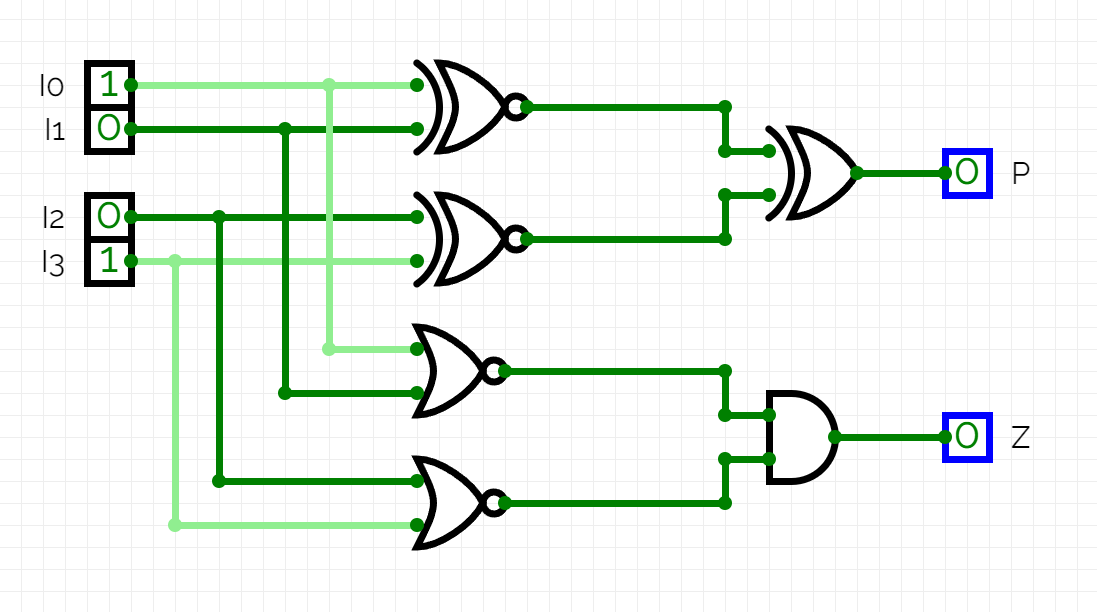
\includegraphics[width=13cm]{images/diagrams/PZ4Esquema.png}
            }
        \caption{Projeção inicial do circuito \textit{PZ4} criado no \textit{Circuitverse\protect\footnotemark}}
    \end{figure}
    \footnotetext{ver referências$^{\ref{Referências}}$ para site}

    \vspace{-.5cm}
    \subsubsection{PZ10}

    \vspace{2mm}
    $P (I0, I1, \cdots, I8, I9) = (\overline{I0 \bigoplus I1})\bigoplus(\overline{I2 \bigoplus I3})\bigoplus(\overline{I4 \bigoplus I5})\bigoplus(\overline{I6 \bigoplus I7})\bigoplus(\overline{I8 \bigoplus I9})$
    %P_{U2}
    
    \vspace{2mm}
    $Z (I0, I1, \cdots, I8, I9) = (\overline{I0 + I1})\cdot(\overline{I2 + I3})\cdot(\overline{I4 + I5})\cdot(\overline{I6 + I7})\cdot(\overline{I8 + I9})$

    
    \begin{figure}[H]
        \centering
            \fbox{%
            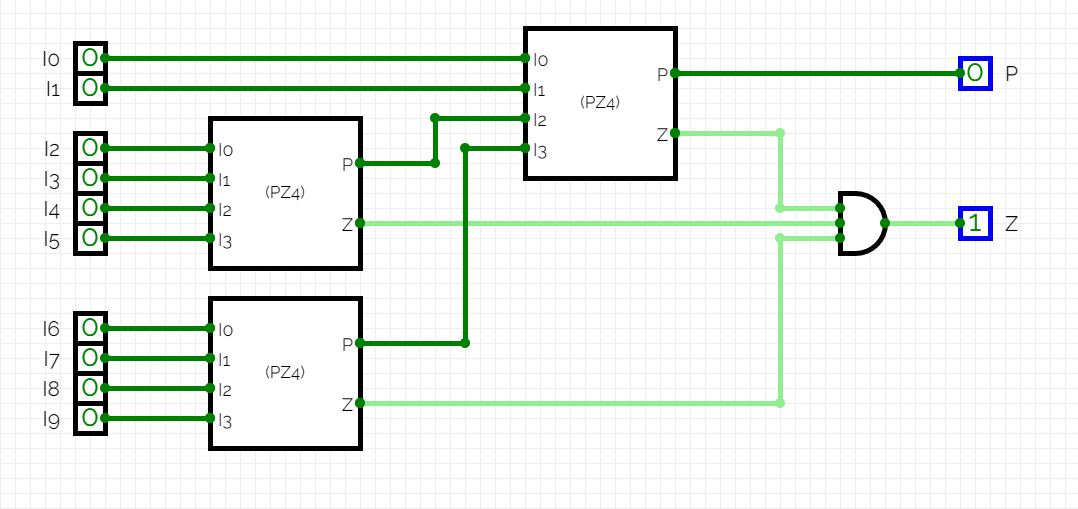
\includegraphics[width=13cm]{images/diagrams/PZ10Esquema.png}
            }
        \caption{Projeção inicial do circuito \textit{PZ10} criado no \textit{Circuitverse\protect\footnotemark}}
    \end{figure}

    \footnotetext{ver referências$^{\ref{Referências}}$ para site}
    
\end{center}

\newpage
\subsection{Simplificação lógica}
\noindent\rule[1.2cm]{3.35in}{.1mm}
\vspace{-0.5cm}

Aplicando as propriedades dos operadores lógicos, conseguimos obter uma simplificação das funções lógicas dos circuitos. \\

Nas funções $P$, $PZ4_{U0}$, $PZ4_{U1}$ e $PZ4_{U2}$, exercemos uma propriedade do \textbf{XNOR}, que, uma vez que a função apresenta dois \textbf{XNORs}, isto é, um par de \textbf{XORs} negados, podemos remover a negação dos \textbf{XNORs} iniciais. E assim ficámos apenas com uma cadeia de \textbf{XORs}, que resultará no mesmo output. \\

No output \textbf{Z}, dos blocos \textit{PZ4}, utilizámos simplesmente as Leis de De Morgan, que passaram de uma soma negada para uma multiplicação de negações, como se pode verificar na função a seguir. \\

A função \textbf{Z}, que funciona como um operador lógico \textbf{AND}, já se encontra simplificada, apenas recebendo como suas entradas, os saídas Z dos três blocos \textit{PZ4} usados neste circuito. O output final \textbf{P} é, precisamente, a saída P do $PZ4_{U2}$.

\vspace{1cm}
\noindent\fbox{%
    \parbox{\textwidth}{%
    \vspace{5mm}
        \large
        \centering

        \textbf{PZ4}

        \vspace{5mm}
        $P (I0, I1, I2, I3) =  (\overline{I0 \bigoplus I1})\bigoplus (\overline{I2 \bigoplus I3}) = I0 \bigoplus I1 \bigoplus I2 \bigoplus I3$

        $Z (I0, I1, I2, I3) = (\overline{I0 + I1}) \cdot (\overline{I2 + I3}) = \overline{I0} \cdot \overline{I1} \cdot \overline{I2} \cdot \overline{I3}$
        \vspace{5mm}
    }%
}

\vspace{1cm}
\noindent\fbox{%
    \parbox{\textwidth}{%
    \vspace{5mm}
    \centering
    \large
        \textbf{PZ10}

        \vspace{5mm}
        $PZ4_{U0}(I2, I3, I4, I5) = (\overline{I2 \bigoplus I3}) \bigoplus (\overline{I4 \bigoplus I5}) = I2 \bigoplus I3 \bigoplus I4 \bigoplus I5$

        $PZ4_{U1}(I6, I7, I8, I9) = (\overline{I6 \bigoplus I7}) \bigoplus(\overline{I8 \bigoplus I9}) = I6 \bigoplus I7 \bigoplus I8 \bigoplus I9$

        $PZ4_{U2}(I0, I1, P_{U0}, P_{U1}) = (\overline{I0 \bigoplus I1}) \bigoplus (\overline{P_{U0} \bigoplus P_{U1}}) = I0 \bigoplus I1\bigoplus P_{U0} \bigoplus P_{U1}$

        
        $P = P_{PZ4_{U2}}$

        
        \vspace{2mm}
        $Z (Z_{U0}, Z_{U1}, Z_{U2}) = Z_{U0} \cdot Z_{U1} \cdot Z_{U2}$

    \vspace{5mm}
    }%
}
\newpage

\subsection{Diagrama de blocos}
\noindent\rule[1.2cm]{3.35in}{.1mm}
\vspace{-1cm}

\begin{figure}[H]
\centering
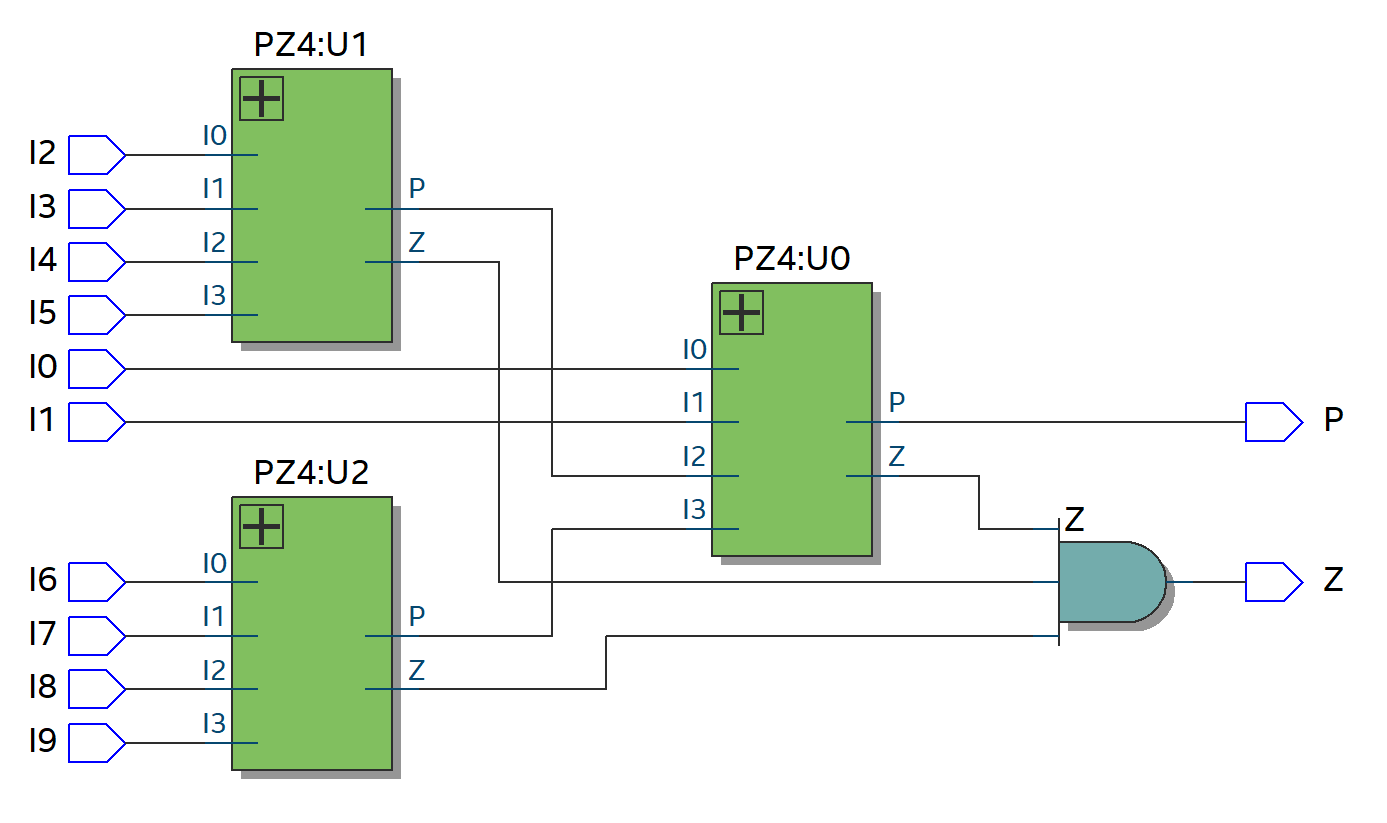
\includegraphics[width=15cm]{images/diagrams/Logigrama.png}
\caption{Diagrama do circuito \textit{PZ10} criado pela funcionalidade \textit{\textbf{RTL Viewer}}}
\end{figure}

\subsection{Atribuição de Pinos}
\noindent\rule[1.2cm]{3.35in}{.1mm}
\vspace{-1cm}

A nossa atribuição aos pinos da placa de teste (\textit{\textbf{DE10-Lite}}) de acordo com os 10 inputs (I0, I1, I2, I3, I4, I5, I6, I7, I8 e I9) e 2 outputs (P e Z) é a seguinte: 
\begin{figure}[H]

    \begin{BVerbatim}
        set_global_assignment -name BOARD "MAX 10 DE10 - Lite"
        set_global_assignment -name DEVICE 10M50DAF484C6GES
        set_global_assignment -name FAMILY "MAX 10"
        set_location_assignment PIN_A8 -to P
        set_location_assignment PIN_A9 -to Z
        set_location_assignment PIN_C10 -to I0
        set_location_assignment PIN_C11 -to I1
        set_location_assignment PIN_D12 -to I2
        set_location_assignment PIN_C12 -to I3
        set_location_assignment PIN_A12 -to I4
        set_location_assignment PIN_B12 -to I5
        set_location_assignment PIN_A13 -to I6
        set_location_assignment PIN_A14 -to I7
        set_location_assignment PIN_B14 -to I8
        set_location_assignment PIN_F15 -to I9
    \end{BVerbatim}
    \caption{Código de atribuição de pinos}
\end{figure}

\newpage

\section{Resultados e Discussão}
\hrule
\vspace{0.5cm}

Logo após a conclusão definitiva do circuito  em \textit{VHDL} dentro do \textit{Quartus}, simulámos, utilizando a ferramenta \textbf{\textit{RTL Simulation}}. Utilizando o \textit{clock}, fomos subdividindo o valor para cada entrada, obtendo assim todas as combinações possíveis de entradas (I0..I9).\\

Verificámos então, que os valores dos outputs (P e Z) correspondentes a cada combinação de inputs, seguiam o proposto pelo guião deste trabalho e sempre apresentaram o valor esperado para quaisquer inputs.
Assim, os resultados obtidos com as simulações do circuito foram os esperados, confirmando que o circuito cumpriu o objetivo inicial.
\subsection{Simulação}
\noindent\rule[1.2cm]{3.35in}{.1mm}
\vspace{-1cm}
\begin{table}[H]
\centering
\begin{tabular}{|c|c|c|c|c|c|c|c|c|c|l|c|c|}

\hhline{----------~--}
\rowcolor{lightgray} \textbf{I0} & \textbf{I1} & \textbf{I2} & \textbf{I3} & \textbf{I4} & \textbf{I5} & \textbf{I6} & \textbf{I7} & \textbf{I8} & \textbf{I9} & {\cellcolor{white}}  & \textbf{P} & \textbf{Z} \\ 

\hhline{----------~--}
1  & 0  & 1  & 0  & 1  & 0  & 0  & 0  & 1  & 1  &  & \cellcolor{green}\textbf{1} & \cellcolor{red}\textbf{0} \\ 

\hhline{----------~--}
1  & 0  & 1  & 0  & 0  & 0  & 1  & 0  & 1  & 0  &  & \cellcolor{red}\textbf{0} & \cellcolor{red}\textbf{0} \\ 

\hhline{----------~--}
1  & 1  & 1  & 1  & 1  & 1  & 1  & 1  & 1  & 1  &  & \cellcolor{red}\textbf{0} & \cellcolor{red}\textbf{0} \\ 

\hhline{----------~--}
0  & 0  & 0  & 0  & 0  & 0  & 0  & 0  & 0  & 0  &  & \cellcolor{red}\textbf{0} & \cellcolor{green}\textbf{1} \\ 

\hhline{----------~--}
\rowcolor{yellow} 0  & 0  & 1  & 1  & 1  & 0  & 1  & 0  & 1  & 1  & \cellcolor[HTML]{FFFFFF} &  \textbf{0} & \textbf{0} \\ 

\hhline{----------~--}
0  & 1  & 1  & 0  & 1  & 1  & 1  & 0  & 1  & 1  &  & \cellcolor{green}\textbf{1} & \cellcolor{red}\textbf{0} \\ 

\hhline{----------~--}
0  & 0  & 0  & 0  & 0  & 0  & 0  & 0  & 1  & 0  &  & \cellcolor{green}\textbf{1} & \cellcolor{red}\textbf{0} \\ 

\hhline{----------~--}
0  & 1  & 0  & 1  & 0  & 1  & 0  & 1  & 0  & 1  &  & \cellcolor{green}\textbf{1} & \cellcolor{red}\textbf{0} \\ 

\hhline{----------~--}
0  & 0  & 1  & 0  & 0  & 1  & 0  & 0  & 1  & 1  &  & \cellcolor{red}\textbf{0} & \cellcolor{red}\textbf{0} \\ 

\hhline{----------~--}
1  & 1  & 0  & 1  & 0  & 1  & 1  & 1  & 0  & 1  &  & \cellcolor{green}\textbf{1} & \cellcolor{red}\textbf{0} \\ 

\hhline{----------~--}
\end{tabular}
\caption{\centering {Combinações\protect\footnotemark} da \textit{Testbench}}
\label{Tabela Simulação}
\end{table}

\footnotetext{O caso indicado a amarelo faz juz à combinação demonstrada pela agulha a amarelo na Figura \ref{SimulaçãoRTL}.}

\vspace*{\fill}
\begin{figure}[H]
\centering
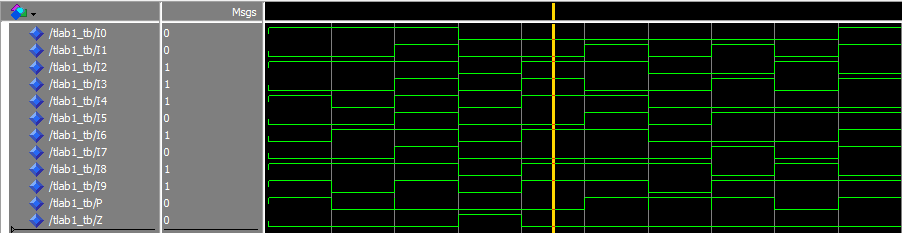
\includegraphics[width=1\linewidth]{images/SimulaçãoRTL.png}
\caption{Visualização dos resultados da \textit{Testbench}}
\label{SimulaçãoRTL}
\end{figure}
\vspace*{\fill}%

\newpage

\subsection{Teste}
\noindent\rule[1.2cm]{3.35in}{.1mm}
\vspace{-1cm}


Apresentamos dois testes distintos, realizados em aula, com a placa \textit{DE10-Lite} :

\vspace*{\fill}
\begin{figure}[H]
    \centering
    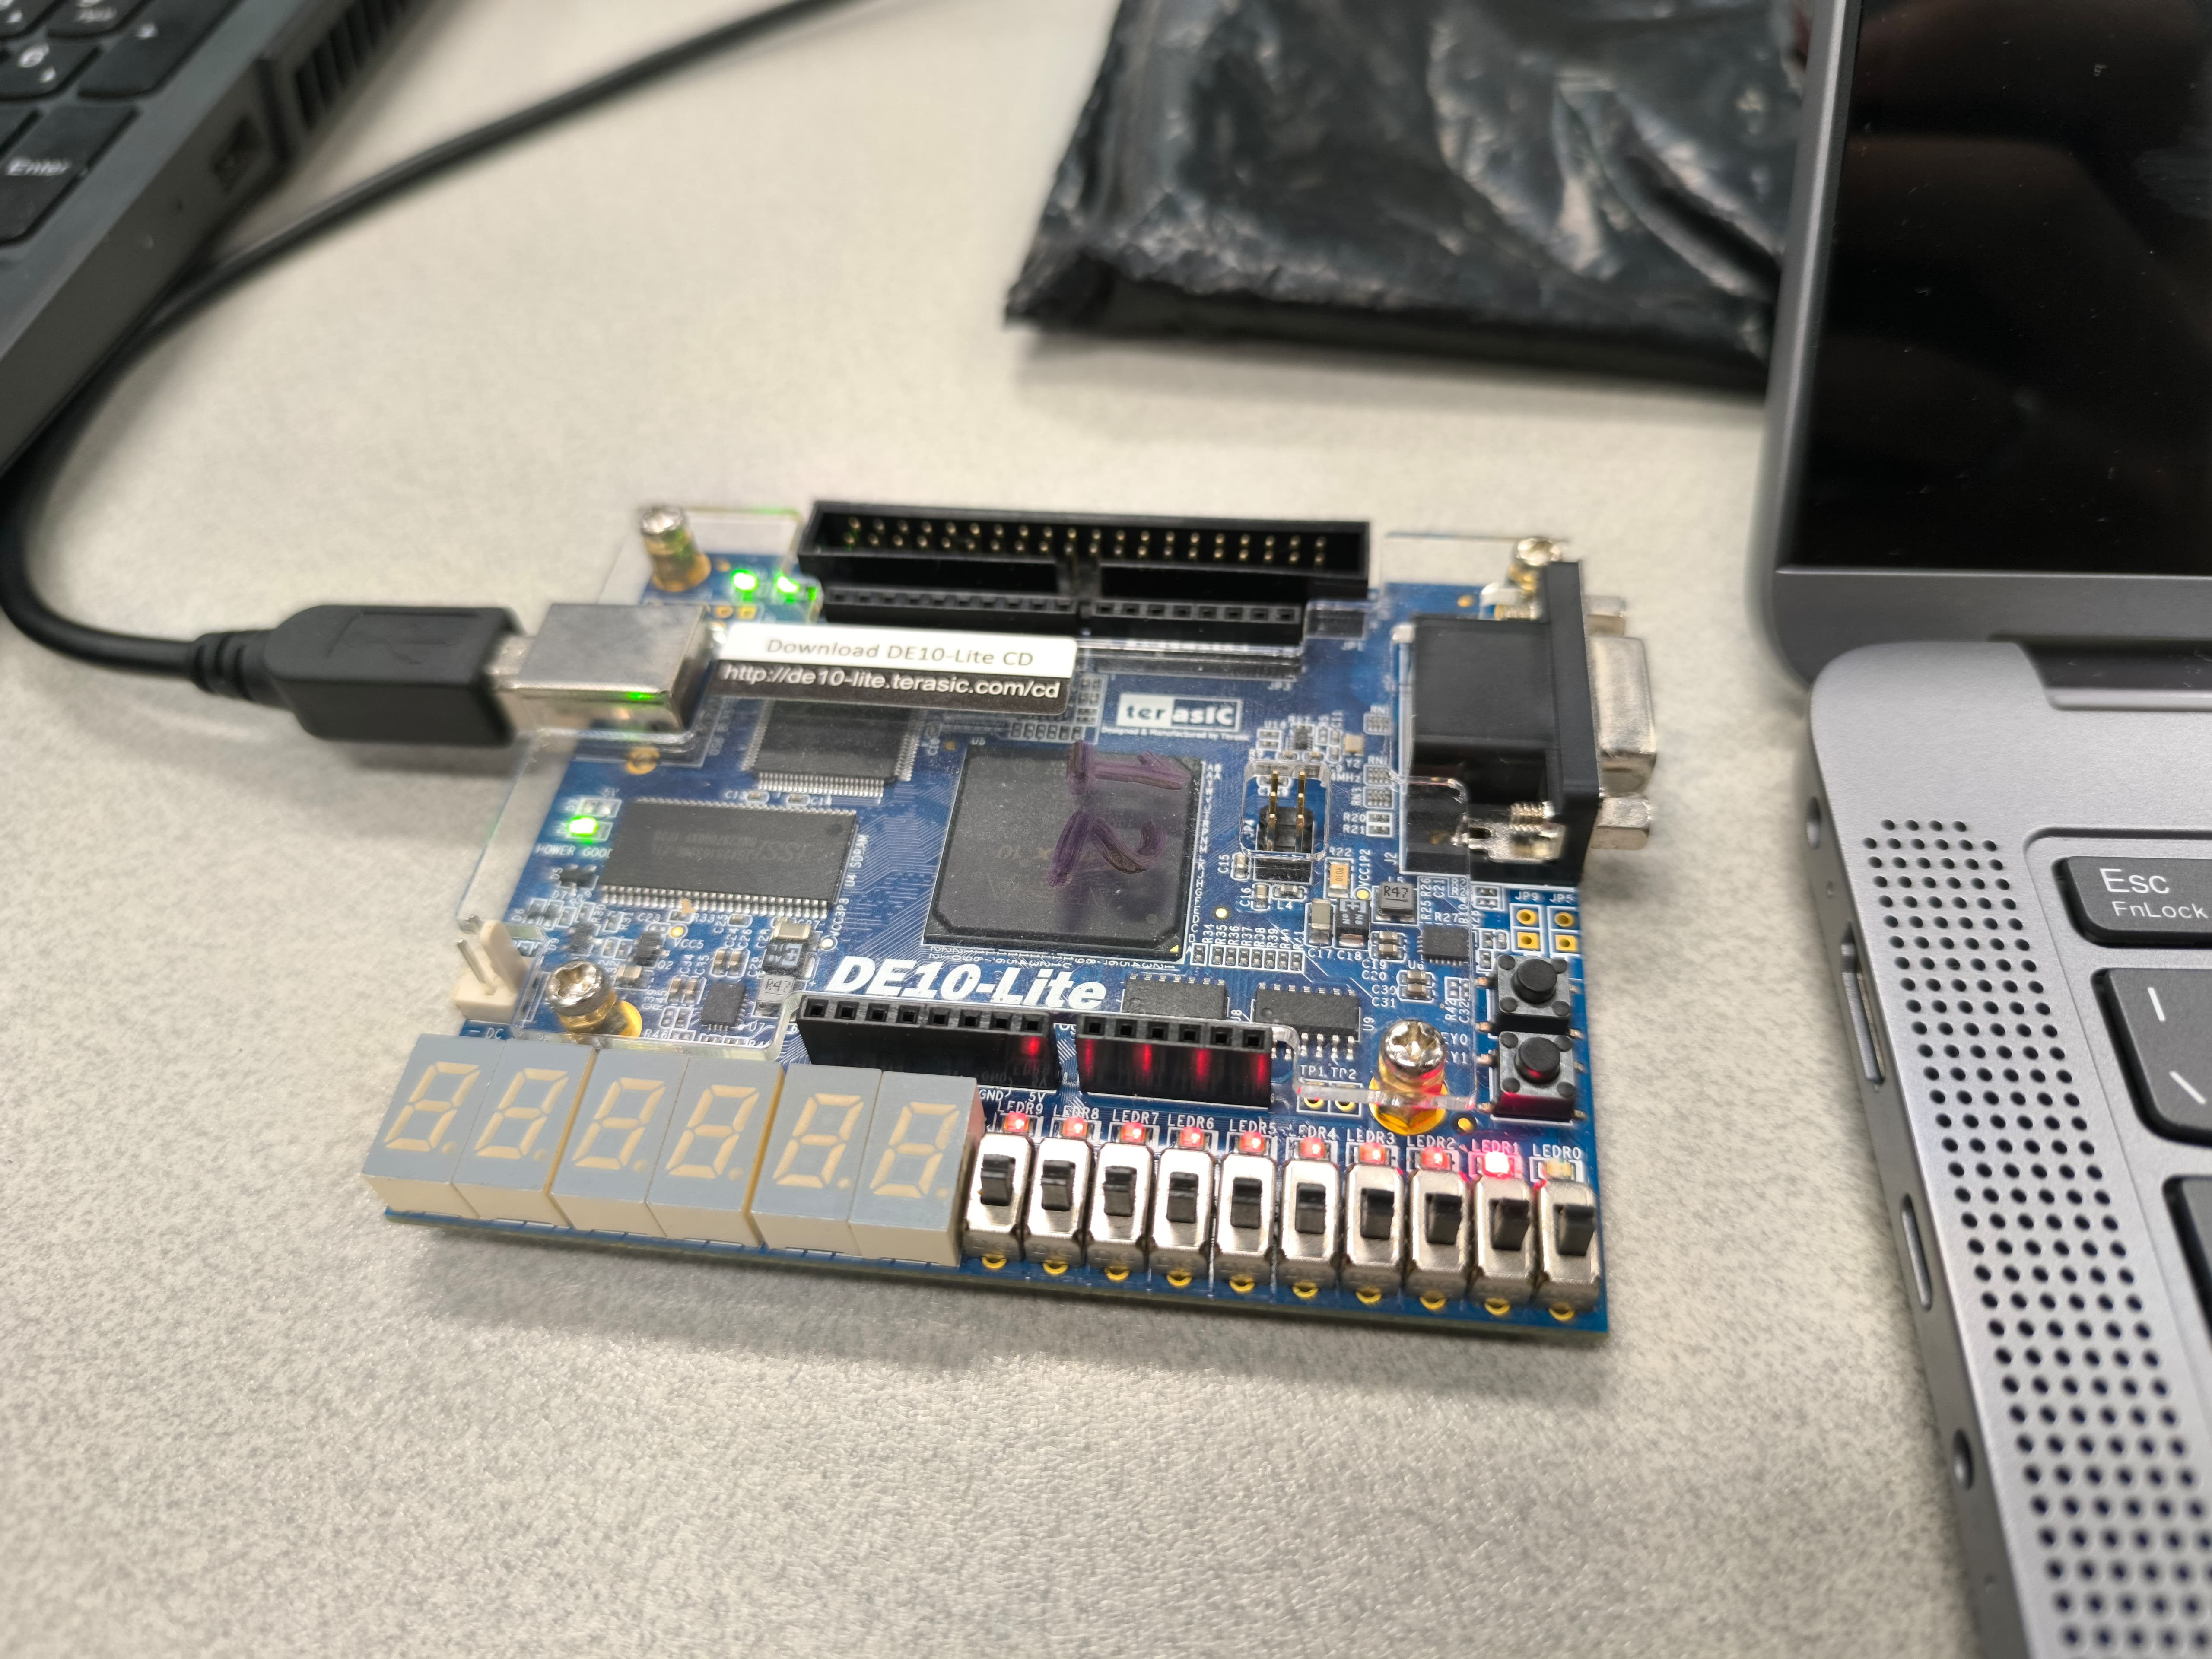
\includegraphics[width=12cm]{images/TesteZero.jpg}
    \caption{Teste para {Zero\protect\footnotemark} \textbf{(Z)}}
    \label{Teste para Zero}
\end{figure}
\footnotetext{Teste com todos os inputs inativos. O último LED corresponde ao output \textbf{P} que se encontra inativo \textbf{(valor 0)}. O penúltimo LED corresponde ao output \textbf{Z} que se encontra ativo \textbf{(valor 1)}}

\begin{figure}[H]
    \centering
    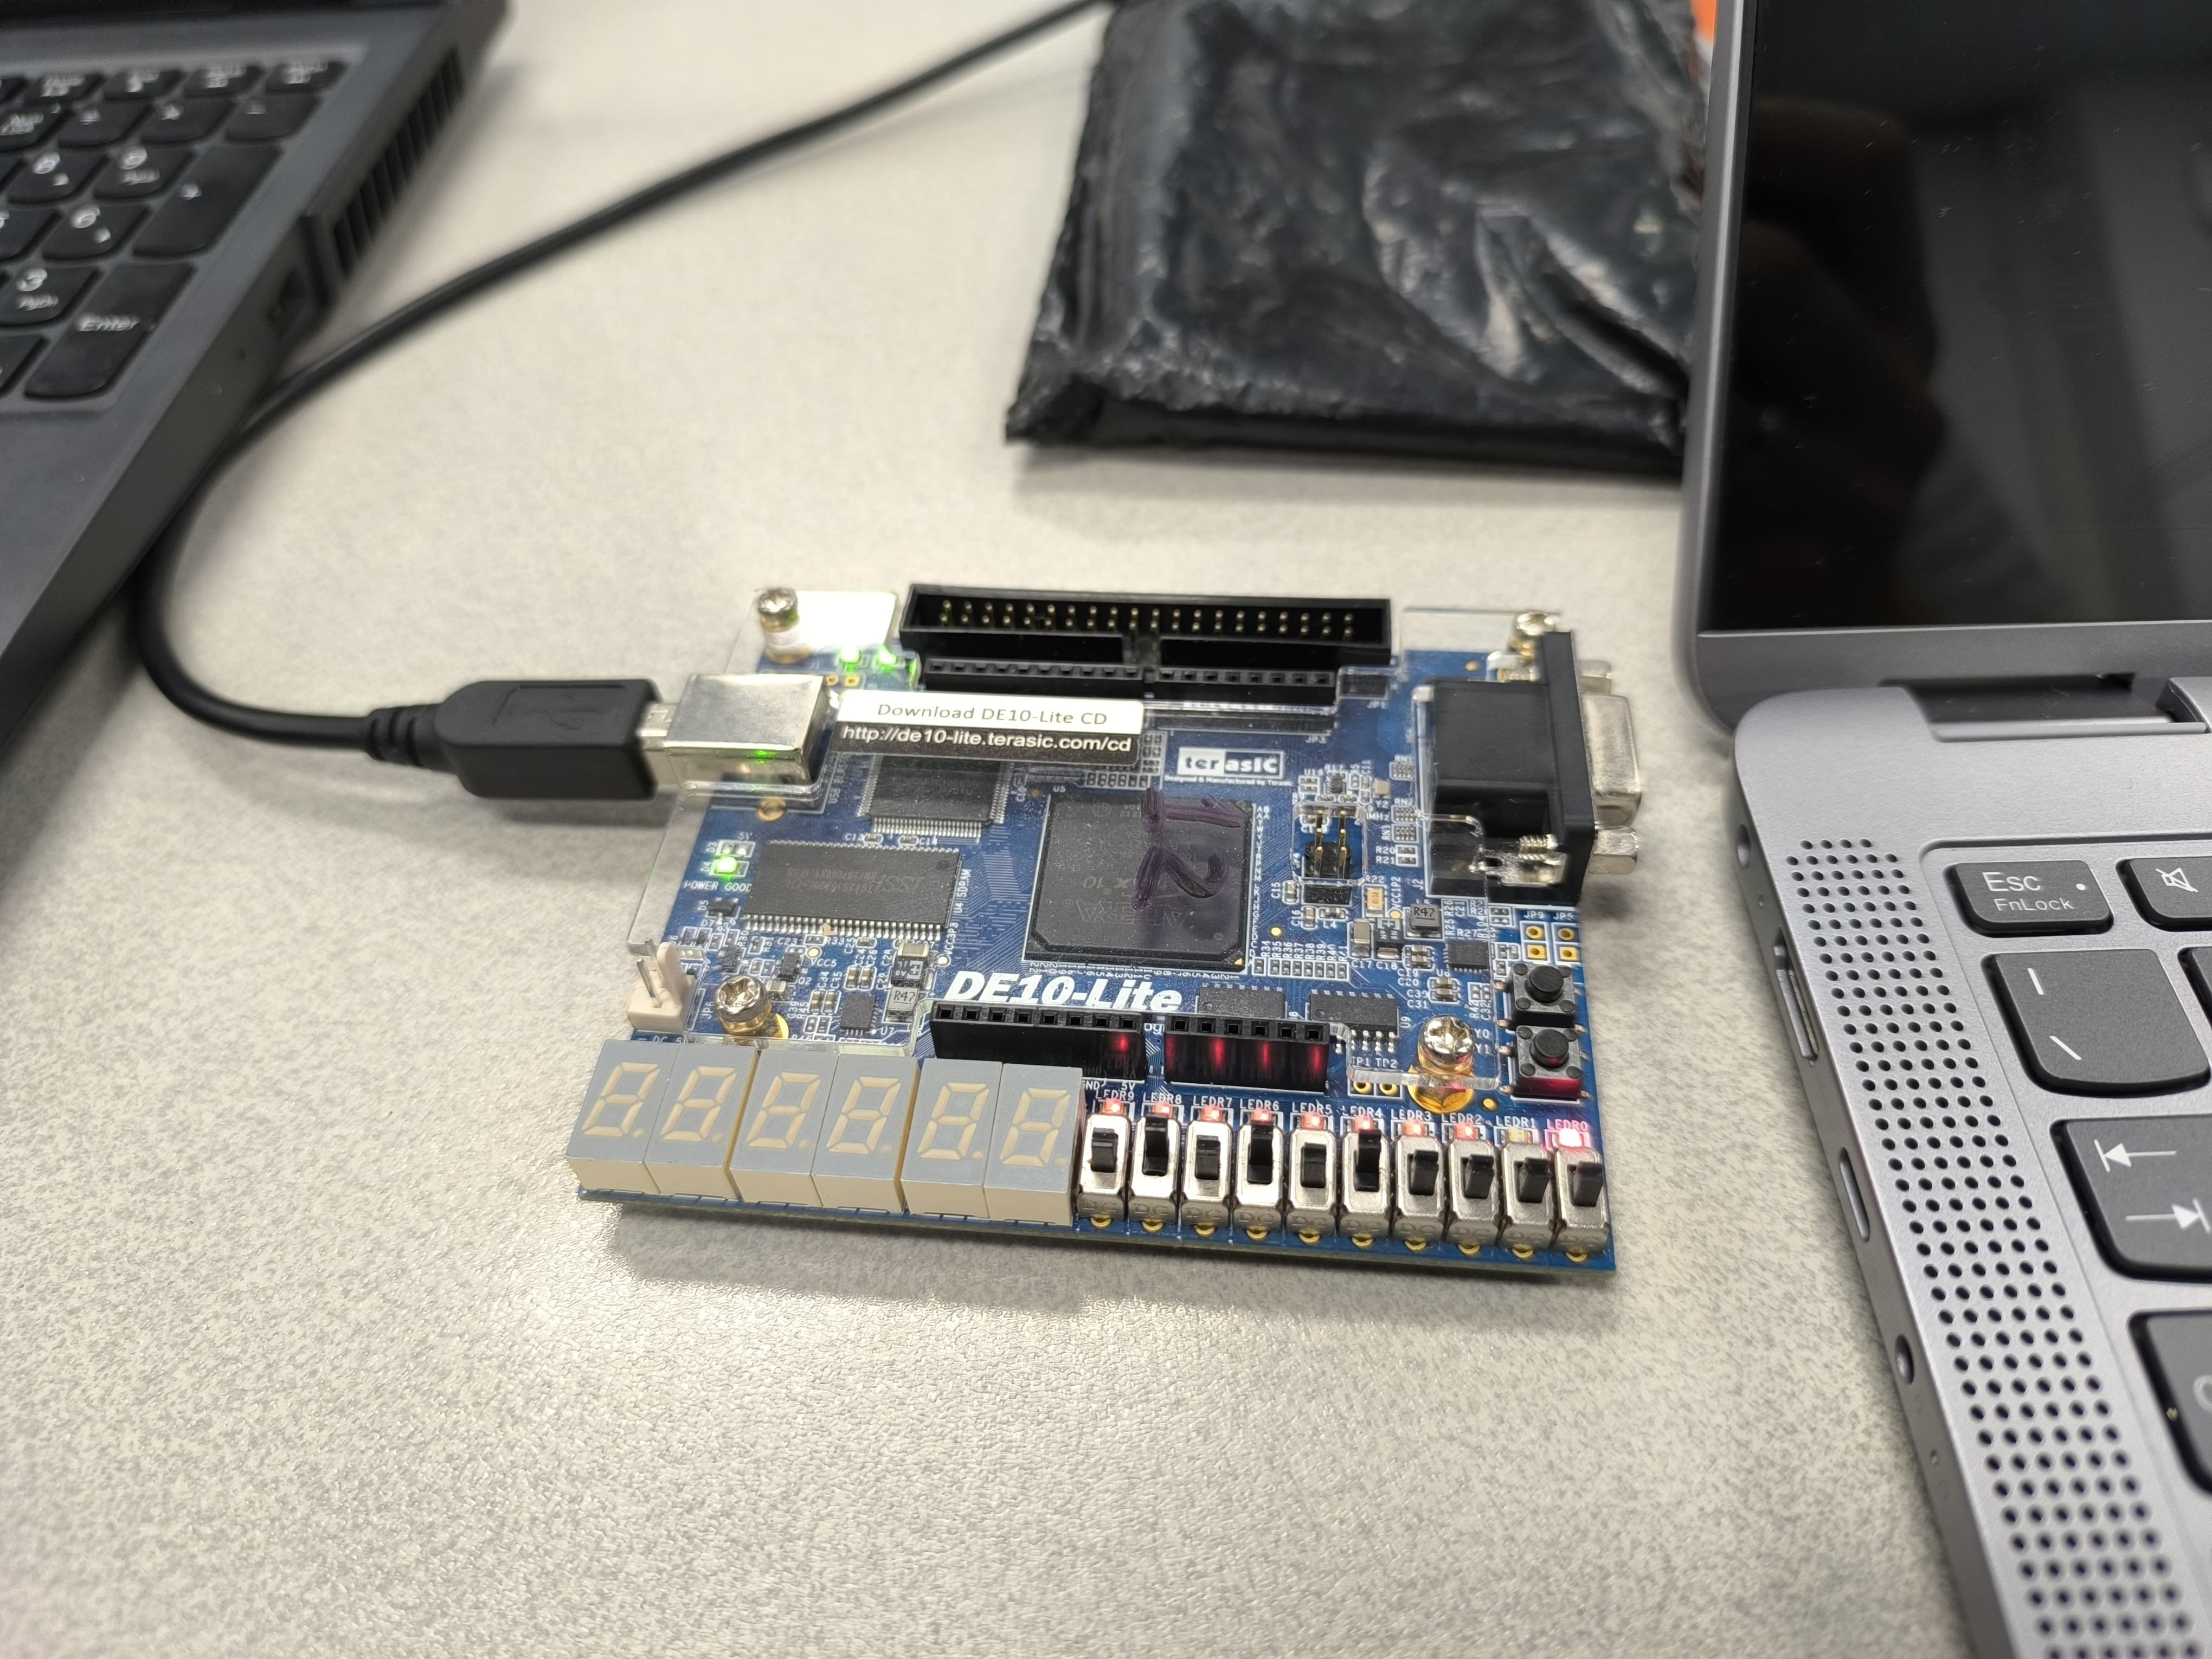
\includegraphics[width=12cm]{images/TesteParidade.jpg}
    \caption{Teste para {Paridade\protect\footnotemark} \textbf{(P)}}
    \label{Teste para Paridade}
\end{figure} 
\footnotetext{Teste com os inputs I5, I7 e I9 ativos. O último LED corresponde ao output \textbf{P} que se encontra ativo \textbf{(valor 1)}. O penúltimo LED corresponde ao output \textbf{Z} que se encontra inativo \textbf{(valor 0)}}
\vspace*{\fill}%

\newpage

\section{Conclusão} 
\hrule
\vspace{0.5cm}
De acordo com os objetivos propostos, concluímos com sucesso o desenvolvimento do circuito destinado à verificação de paridade e estado nulo das entradas. Através da utilização da linguagem \textbf{\textit{VHDL}} no software \textbf{\textit{Quartus}} da \textbf{\textit{Intel}}, aliada à implementação prática na placa \textbf{\textit{DE10-Lite}}, foi possível desenvolver um \textbf{circuito} que responde de forma \textbf{eficaz} e \textbf{precisa} aos critérios estabelecidos. \\

O circuito verifica a paridade das entradas, ativando o output \textbf{P} quando o número de entradas ativas \textbf{(valor 1)} é \textbf{ímpar}, e, adicionalmente, garante a ativação do output \textbf{Z} sempre que \textbf{não há} entradas ativas.\\

Ao longo do processo, procedemos a uma fase intensiva de testes na placa \textit{DE10-Lite}, os quais confirmaram a \textbf{exatidão} do funcionamento do circuito. Os resultados experimentais foram consistentes e corroboraram plenamente as expectativas iniciais, \textbf{validando} a implementação do circuito e \textbf{confirmando} a correção dos outputs \textbf{P} e \textbf{Z} nas diferentes condições de entrada testadas.\\

Além de termos cumprido as especificações fornecidas no guião, esta experiência permitiu-nos \textbf{aprofundar} conhecimentos sobre a \textbf{aplicação prática} de circuitos digitais em contextos de \textbf{verificação} de paridade e \textbf{detecção} de entradas nulas. O projeto também nos proporcionou um maior domínio das ferramentas de desenvolvimento \textit{\textbf{VHDL}} e da plataforma \textit{\textbf{Quartus}}, ao mesmo tempo que reforçou a nossa capacidade de \textbf{interpretar} e \textbf{implementar} soluções de acordo com as especificações exigidas.\\

Em suma, o trabalho realizado não só \textbf{cumpriu} os requisitos teóricos e práticos propostos, como também ampliou a nossa compreensão sobre a relevância e a eficácia dos circuitos digitais em problemas reais de verificação lógica.
 


%O trabalho consistiu em elaborarmos um circuito que verificasse a paridade dos inputs, isto é, verificar se o número de entradas ativas \textbf{(1)} é ímpar, e no caso afirmativo, o output P estaria ativado \textbf{(1)}. Caso contrário, se o número de entradas ativas \textbf{(1)} é par, o output P desativar-se-ia \textbf{(0)}. Por outro lado, o nosso circuito tinha também de verificar se o número de entradas ativas \textbf{(1)} era nulo, e no caso de isto se verificar, o output Z estaria ativo \textbf{(1)}. Qualquer outra situação, onde pelo menos um input esteja ativo \textbf{(1)}, o output Z surge desativado \textbf{(0)}.\\ %Foi desenvolvido em linguagem \textbf{VHDL} no programa \textit{Quartus} da Intel. \\ %Foi testado na placa \textit{\textbf{DE10-Lite}} da Intel.\\ %Os resultados experimentais confirmam o funcionamento do circuito de acordo com o pretendido desde o início. Conseguimos compreender o problema em causa, e aplicar um circuito eficiente que faz juz às indicações fornecidas no guião, relativamente à \textbf{Paridade} e \textbf{Zero} apresentadas no mesmo.


%-------------------------------------------------------------------------------
% REFERENCES
%-------------------------------------------------------------------------------
\newpage
\pagestyle{referencias}

\section*{Referências} \label{Referências}
\addcontentsline{toc}{section}
{\protect\numberline{}Referências}
\hrule
\vspace{0.5cm}

\begin{itemize}
    \item \href{https://circuitverse.org/}{\textbf{Circuitverse}}: Usado para a simulação inicial e esquematização do circuito;
    
    \item \textbf{\href{https://www.overleaf.com/learn}{\textbf{Overleaf Documentation}}}: Usada em recurso para desenvolvimento do documento em \textit{LaTeX};
    
    \item \href{https://www.cmor-faculty.rice.edu/~heinken/latex/symbols.pdf}{\textbf{Rice University \textit{LaTeX} Mathematical Symbols}}: Documento da Universidade Rice, no Texas, dedicado demonstrar símbolos e técnicas de formatação em \textit{LaTeX} menos usados e que nos muito útil ao desenvolvimento do documento;
    
    \item \href{https://www.math.uci.edu/~xiangwen/pdf/LaTeX-Math-Symbols.pdf}{\textbf{UC Irvine Department of Mathematics \textit{LaTeX} Math Symbols}}: Documento da Universidade da Califórnia, na cidade de Irvine, que contém uma compilação de símbolos, gráficos, tabelas e entre outros muito úteis para o desenvolvimento deste documento em \textit{LaTeX};
    
    \item \href{https://2425moodle.isel.pt/pluginfile.php/1261036/mod_folder/content/0/VHDL%20parte2.pdf?forcedownload=0}{\textbf{\textit{VHDL} Estrutural e Simulação - Professor Mário Véstias}}: Material disponibilizado pelo Professor Mário Véstias, do ISEL. Este documento serve como referência para o desenvolvimento de modelos estruturais e a realização de simulações em \textit{VHDL};

    \item \href{https://2425moodle.isel.pt/pluginfile.php/1254903/mod_folder/content/0/Aula%20T4%20-%20Mapas%20de%20Karnaugh.pdf?forcedownload=0}{\textbf{Simplificação Lógica: Método de Karnaugh - Professor Mário Véstias}}: Documento fornecido pelo Professor Mário Véstias, do ISEL, utilizado para explicar o processo de simplificação lógica através dos Mapas de Karnaugh.

\end{itemize}

\newpage
\pagestyle{geral}

\appendix
\section{VHDL}
\hrule
\vspace{1cm}

\subsection{PZ4.vhd}
\noindent\rule[1.2cm]{3.35in}{.1mm}
\vspace{-0.5cm}

\begin{minipage}{\linewidth}
    \large\inputminted{vhdl}{PZ4.vhd}
\end{minipage}

\newpage

\subsection{PZ10.vhd}
\noindent\rule[1.2cm]{3.35in}{.1mm}
\vspace{-0.5cm}

\begin{minipage}{\linewidth}
    \inputminted{vhdl}{PZ10.vhd}
\end{minipage}

\newpage
\section{Esquema Elétrico}
\hrule
\vspace{0.5cm}

\vspace*{\fill}
\begin{figure}[H]
\centering
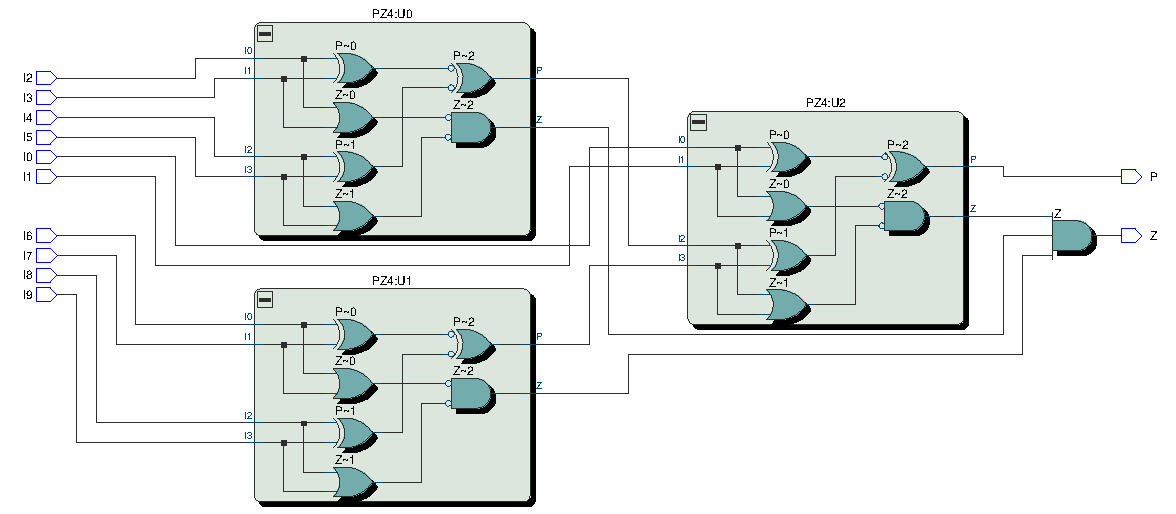
\includegraphics[angle=0,width=1\linewidth]{images/diagrams/EsquemaElétrico.pdf}
\caption{Esquema elétrico do circuito \textit{PZ10}}
\end{figure}
\vspace*{\fill}%

\newpage
\section{Índice Remissivo}
\pagestyle{remissivo}
\hrule
\vspace{0.5cm}

\listoffigures
\listoftables

\end{document}